%%%%%%%%%%%%%%%%%%%%%%%%%%%%%%%%%%%%%%%%%%%%%%%%%%%%%%%%%%%%%%%%%%%%%%%%
\chapter{Preliminaries}
%%%%%%%%%%%%%%%%%%%%%%%%%%%%%%%%%%%%%%%%%%%%%%%%%%%%%%%%%%%%%%%%%%%%%%%%

\section{Graphs}
\label{sec:prelim-graphs}
% Define graphs (weights and edge directions).
% Neighbors, out/in-neighbors, degree
% Graph and network (network mainly for real scenarios e.g., social, citation, road network...)
A graph\footnote{In the literature, graphs representing real-world phenomena
are often called \enquote{networks} -- \eg social networks, road networks,
\etc We use these two names interchangeably. Further, in the context of
graphs, the names \enquote{node} and \enquote{vertex} are often used
as synonyms. We use \enquote{vertex} for an element in $V$ and we reserve
\enquote{node} for computing units in a distributed memory system.} is an ordered
pair $(V, E)$ where $V$ is the set of vertices, $E \subseteq V\times V$ is the
set of edges, $n = |V|$ is the number of vertices, and $m = |E|$ is the number
of edges.
A graph $G = (V, E)$ is a \emph{subgraph} of another graph $G' = (V', E')$ if
$G$ contains all the vertices and edges of $G'$, \ie
$V \subseteq V'$ and $E \subseteq E' \cap (V \times V)$.

An edge $e = \set{u, v} \in E$ is
\emph{incident} to $u$ and $v$ and both vertices are \emph{adjacent} to
each other.
The \emph{neighborhood} of a vertex $u$ is the set of
vertices adjacent to $u$, \ie $N(u) := \set{v \in V\ |\ \set{u, v} \in E}$. The
vertices in $N(u)$ are also called the \emph{neighbors} of $u$. The
\emph{degree} of a vertex $u$, denoted $\deg(u)$, is the cardinality of its
neighborhood.

\sloppy
If edges are ordered sets of pairs then the graph is called \emph{directed}
and we denote by $(u, v)$ an edge \emph{from} a vertex $u$ \emph{to} a vertex $v$;
otherwise, the graph is called \emph{undirected} -- \Cref{fig:undirected-graph}
and \Cref{fig:directed-graph} show an example of an undirected graph
and a directed graph, respectively.
In directed graphs, a vertex $u$ has \emph{out}-neighbors, \ie the set of
vertices $\nout(u) := \set{v\in V\ |\ (u, v) \in E}$, and \emph{in}-neighbors, \ie
$\nin(u) := \set{v\in V\ |\ (v, u) \in E}$; the neighbors of $u$ is the union of $u$'s
out-neighbors and in-neighbors: $N(u) := \nout(u) \cup \nin(u)$.
The cardinalities $\degout(u) :=
|\nout(u)|$, $\degin(u) := |\nin(u)|$, and $\deg(u) := |N(u)|$ are called
\emph{out}-degree, \emph{in}-degree, and degree of $u$, respectively.

A \emph{weighted} graph is an ordered triplet $(V, E, w)$ where $(V, E)$ is
an unweighted graph and $w$ is the \emph{weight} function, \ie $w : E
\rightarrow \real$. In weighted graphs, the degree can be extended to the sum of
the weights of the (in/out) neighbors, namely the \emph{weighted degree} and
the \emph{weighted in-} and \emph{out-degree}.
In this thesis, we only consider strictly positive edge weight functions. An
unweighted graph can also be interpreted as a weighted graph with weight
function $w : E \rightarrow 1$, \ie every edge has weight 1.

\begin{figure}[tb]
\centering
\begin{subfigure}[t]{.4\textwidth}
\centering
\begin{tikzpicture}
\vertex{-1,1}{0}{0}
\vertex{1,1}{1}{1}
\vertex{0,0}{2}{2}
\vertex{-1,-1}{3}{3}
\vertex{1,-1}{4}{4}

\edge{0}{3}
\edge{1}{2}
\edge{1}{4}
\edge{2}{3}
\edge{2}{4}
\edge{3}{4}
\end{tikzpicture}

\caption{Example of undirected graph with $n = 5$ vertices
and $m = 6$ edges.}
\label{fig:undirected-graph}
\end{subfigure}\hfill
\begin{subfigure}[t]{.4\textwidth}
\centering
\begin{tikzpicture}
\vertex{-1,1}{0}{0}
\vertex{1,1}{1}{1}
\vertex{0,0}{2}{2}
\vertex{-1,-1}{3}{3}
\vertex{1,-1}{4}{4}

\dedge{0}{3}
\dedge{1}{2}
\dbedge{1}{4}{bend left=20}
\dbedge{4}{1}{bend left=20}
\dedge{2}{3}
\dedge{2}{4}
\dedge{3}{4}
\end{tikzpicture}


\caption{Example of directed graph with $n = 5$ vertices
and $m = 7$ edges.}
\label{fig:directed-graph}
\end{subfigure}
\caption{Examples of undirected and directed graphs.}
\end{figure}

\paragraph{Matrix Representations of a Graph}
A graph $G = (V, E, w)$ can be represented using matrices. In this work,
matrices are denoted by bold capital letters such as \mat{M} and the element
at the $i$-th row and $j$-th column of \mat{M} by $\mat{M}[i, j]$. Similarly,
we type vectors as bold lowercase letters such as $\vect{v}$ and we denote the
element at index $i$ in $\vect{v}$ by $\vect{v}[i]$. The \emph{adjacency
matrix} \Adj of $G$ is a square $n \times n$ matrix such that $\Adj[u,v] = w(u,
v)$ if there is an edge from $u$ to $v$, zero otherwise. Clearly, if $G$ is
undirected, then \Adj is symmetric. The \emph{Laplacian matrix} \Lapl of $G$ is
defined as:
%
\[\Lapl := \Deg - \Adj,\]
%
where \Deg is the \emph{degree matrix} of $G$, \ie the diagonal matrix
such that $\Deg[u,u]$ is the (possibly weighted) degree of $u$.
If $G$ is undirected, then $\Lapl$ is symmetric and positive-semidefinite.
For example, the adjacency and the Laplacian matrices of the graph
in \Cref{fig:undirected-graph} are respectively:
%
\[
\Adj =
\begin{pmatrix}
0 & 0 & 0 & 1 & 0\\
0 & 0 & 1 & 0 & 1\\
0 & 1 & 0 & 1 & 1\\
1 & 0 & 1 & 0 & 1\\
0 & 1 & 1 & 1 & 0\\
\end{pmatrix}\hspace{5mm}
\text{and}\hspace{5mm}
\Lapl =
\begin{pmatrix}
1 & 0 & 0 & -1 & 0\\
0 & 2 & -1 & 0 & -1\\
0 & -1 & 3 & -1 & -1\\
-1 & 0 & -1 & 3 & -1\\
0 & -1 & -1 & -1 & 3\\
\end{pmatrix}.
\]

%%%%%%%%%%%%%%%%%%%%%%%%%%%%%%%%%%%%%%%%%%%%%%%%%%%%%%%%%%%%%%%%%%%%%%%%
%
\section{Paths and Components}
%
\begin{definition}[Walk, Trail and Path]
A walk on a graph $G = (V, E, w)$ is an alternating sequence of vertices
$(u_0, u_1, \ldots, u_\ell)$ and edges $(e_1, e_2, \ldots, e_\ell)$
where $e_i = (u_{i - 1}, u_i) \in E$ for all $0 < i \le \ell$.
The number $\ell$ of edges in the walk is called the \emph{length} of the walk.
A \emph{trail} is a walk where all edges are distinct and a \emph{path}
is a walk with distinct vertices.
\end{definition}

\begin{definition}[Random Walk]
\label{def:random-walk}
A random walk of length $\ell$ on a graph $G = (V, E, w)$ is a walk $(u_0,
u_1, \ldots, u_\ell)$ obtained in a random fashion. Starting at vertex $u_0$,
its next vertex $u_1$ is chosen at random from $u_0$'s (out) neighbors, and so
on.
\end{definition}

Hereafter, we denote $P_{s,t}$ a path where $s = u_0$ and $t = u_\ell$.
Additionally, a \change{\emph{circuit} is a trail where $u_0 = u_\ell$ and
a \emph{cycle} is a circuit with no repeated vertices}.
If a graph does not have cycles it is called \emph{acyclic}. Directed
acyclic graphs are abbreviated with the acronym DAG.

On weighted graphs, the weight of a walk $W$ is defined as the sum of the
weights of the edges it traverses:

\[
w(W) := \sum_{i = 1}^\ell w(e_i).
\]

Clearly, if the graph is unweighted, the length and the weight of a walk
coincide.\footnote{Recall that an unweighted graph is also a weighted graph where
all edges have weight 1.}

If there exists a path from a vertex $s$ to a vertex $t$, we say that $s$
\emph{reaches} $t$ or, alternatively, that $t$ is \emph{reachable} from $s$.
Reachability is important to determine connectivity and the components in a
graph.

\begin{definition}[Connected Graph]
An undirected graph is \emph{connected} if any vertex reaches any other vertex.
\end{definition}

\begin{definition}[Connected Component]
A \emph{connected component} (or CC) of a graph $G$ is a maximal connected subgraph
$C$ of $G$, \ie no additional vertex or edge can be added to $C$ without
breaking its property of being connected.
\end{definition}

Clearly, a connected graph has only one connected component -- \eg the graph in
\Cref{fig:undirected-graph} is connected.
Moreover, we call \emph{tree} an undirected acyclic connected graph and \emph{forest}
a disjoint union of trees.

\begin{definition}[Strongly Connected Graph]
A directed graph is \emph{strongly connected} if any vertex reaches any other
vertex.
\end{definition}

\begin{definition}[Strongly Connected Component]
A \emph{strongly connected component} (or SCC) of a directed graph $G$ is a
maximal strongly connected subgraph of $G$.
\end{definition}

For example, the graph in \Cref{fig:directed-graph} has three SCCs:
$\set{\set{0}, \set{3},\set{1, 2, 4}}$. Analogously to the undirected case,
strongly connected graphs consist of only one strongly connected component.
By ignoring edge directions in directed graphs, we also have \emph{weakly connected graphs}
and \emph{weakly connected components}.

\begin{definition}[Weakly Connected Graph]
A directed graph is \emph{weakly connected} all vertices are connected to each
other by a path that ignores edge directions.
\end{definition}

\begin{definition}[Weakly Connected Component]
A \emph{weakly connected component} (or WCC) of a directed graph $G$ is a
maximal weakly connected subgraph of $G$.
\end{definition}

For example, the graph in \Cref{fig:directed-graph} is weakly connected because
it has only one weakly connected component.
%
Finally, we introduce biconnectivity, \ie the property of graphs to remain
connected after the removal of a vertex.

\begin{definition}[Biconnected Graph]
A [directed] graph is \emph{biconnected} if it remains [strongly] connected
after the removal of any one vertex.
\end{definition}

\begin{definition}[Biconnected Component]
A \emph{biconnected component} of a graph $G$ is a
maximal biconnected subgraph of $G$.
\end{definition}

Clearly, the graph in \Cref{fig:undirected-graph} is not biconnected --
the removal of vertex 3 splits the graph into two connected components --
but it has two biconnected components: $\set{\set{0, 3}, \set{1, 2, 3, 4}}$.


%%%%%%%%%%%%%%%%%%%%%%%%%%%%%%%%%%%%%%%%%%%%%%%%%%%%%%%%%%%%%%%%%%%%%%%%
%
\section{Distances in Graphs}
\label{sec:distances-in-graphs}
% Shortest-path distance
% Resistance distance
% Forest distance
In mathematics, a \emph{metric} on a set $S$ is a function $d : S \times S \rightarrow \real_{\ge 0}$
that satisfies the following axioms for all $x, y, z \in S$:
\begin{enumerate}
    \item identity of indiscernibles: $d(x, y) = 0 \iff x = y$;
    \item symmetry: $d(x, y) = d(y, x)$;
    \item triangle inequality: $d(x, y) \le d(x, z) + d(z, y)$.
\end{enumerate}

We call such a function a \emph{distance function}.
Also, we define the distance between a point $s \in S$
and a subset $P \subseteq S$ as the distance from $s$ to the nearest point in
$P$:

\begin{equation}
\label{eq:def:dist-point-set}
d(s, P) := \min_{p \in P}d(s, p).
\end{equation}

In an undirected graph $G = (V, E, w)$ with positive edge weights,
the \emph{vertex distance} is a metric $d: V\times V \rightarrow \real_{\ge 0}$
defined on all the pairs of vertices in $G$.
Notwithstanding that the symmetry property does not necessarily hold in
directed graphs, we follow the standard convention and use the term
\enquote{distance} even in the directed case.
We now introduce three vertex distance measures that are necessary for the
definition of the centrality measures described in
\Cref{sec:centrality-measures,sec:group-centrality-measures}.


%%%%%%%%%%%%%%%%%%%%%%%%%%%%%%%%%%%%%%%%%%%%%%%%%%%%%%%%%%%%%%%%%%%%%%%%
%
\subsection{Shortest-path Distance}
%
The shortest-path distance, also known as the \emph{geodesic} distance,
is one of the most natural and common definitions of vertex distance in graphs.
The \emph{shortest path} between two vertices $s$ and $t$ is the path $P_{s,t}$
with minimum weight -- note that such a path might not be unique.

\begin{definition}[Shortest-path Distance]
The \emph{shortest-path distance} is the function
$d : V \times V \rightarrow \real_{\ge 0}$ such that $d(s, t)$
is the weight of the path $P_{s,t}$ with minimum weight.
\end{definition}

Conventionally, if $t$ is not reachable from $s$, the distance $d(s, t)$ is
defined as infinite.

\begin{definition}[Diameter]
The \emph{diameter} of a graph of a graph $G$ is the maximum
shortest-path distance between two reachable vertices $u$ and $v$ where $u$
reaches $v$:
%
\[\diam(G) := \max_{\substack{u,v\in V,\\d(u, v) < +\infty}}d(u, v).\]
\end{definition}

\begin{definition}[Eccentricity]
The \emph{eccentricity} of a vertex $u \in V$ is the maximum shortest-path
distance from $u$ to a vertex $v$ reachable from $u$:
\[\ecc(u) := \max_{\substack{v\in V,\\d(u, v) < +\infty}} d(u, v).\]
\end{definition}


Computing the shortest path between two vertices is a classic problem in
algorithmic graph theory and can be solved by the well-known Dijkstra's
algorithm in $\Oh(m + n\log n)$ time -- if the priority queue is implemented
using a Fibonacci Heap.
The same algorithm can also solve the more general \emph{Single-Source Shortest Path}
problem (or SSSP), \ie finding the shortest distances from a vertex to \emph{all}
the other vertices in a graph, in $\Theta(m + n\log n)$ time. If the graph is
unweighted, both the shortest path and the SSSP problems can be solved in $\Oh(n +
m)$ time with a Breadth-First Search (or BFS). The problem of computing the
shortest-path distances between all pairs of vertices is known as the
\emph{All-Pairs Shortest Path} problem (or APSP), and can be solved in $\Oh(nm +
n^2\log n)$ time by \change{running Dijkstra's algorithm from each vertex or
-- for graphs with arbitrary edge weights --} Johnson's algorithm. On
unweighted graphs, in turn, it suffices to run a BFS from each vertex, which
requires $\Theta(n^2 + nm)$ time.

In addition to the aforementioned \emph{combinatorial} techniques,
shortest-path distance problems can also be solved algebraically via
\emph{matrix multiplication}. APSP can be solved in $\Oh(n^\omega \log n)$ by
repeatedly squaring the adjacency matrix of a graph, where $\omega <
\numprint{2.373}$~\cite{DBLP:conf/soda/AlmanW21}
is the matrix multiplication exponent, \ie the smallest constant such that the
product of two $n\times n$ matrices can be performed within $\Oh(n^{\omega +
o(1)})$ algebraic operations.
The logarithmic factor of the time complexity can be saved by a recursive
decomposition of the problem~\cite[Theorem 5.7, p. 204]{DBLP:books/aw/AhoHU74}.
In case of integral edge weights, further improvements have been proposed
for undirected~\cite{DBLP:conf/focs/ShoshanZ99} and directed graphs
\cite{DBLP:conf/focs/Zwick98,DBLP:conf/stoc/Zwick99}.
Despite being asymptotically faster than combinatorial algorithms on dense
graphs,\footnote{The \emph{density} of a graph is $m / {n \choose 2}$,
\ie the fraction of edges actually present in the graph over the maximum
possible number of edges. Consider a sequence of graphs of increasing number
of vertices $n$. If the density approaches zero as $n$ becomes large, the
graphs are said to be \emph{sparse}. Otherwise, a graph where the density
remains non-zero in the limit of large $n$ is said to be
\emph{dense}. Clearly, we cannot take the limit of real-world networks and thus
we cannot determine formally whether they are sparse or dense.
Informally, however, for these networks \enquote{sparse} means that most of
the edges that could exist in the network are not present~\cite[Section
6.10.1]{newman2018networks}.}
methods based on matrix multiplication are in practice not applicable to large
graphs because they require to store dense matrices.


%%%%%%%%%%%%%%%%%%%%%%%%%%%%%%%%%%%%%%%%%%%%%%%%%%%%%%%%%%%%%%%%%%%%%%%%
%
\subsection{Resistance Distance}
\label{sec:prelim-resistance-distance}
%
In the context of determining the distance between two vertices in a graph,
some applications require to take into account not only the \emph{shortest} paths,
but \emph{all} the paths between the two
vertices~\cite{DBLP:journals/socnet/Borgatti05,
DBLP:journals/corr/abs-math-0602073,stephenson1989rethinking}.
A typical example are
electrical networks: an electrical network can be
regarded as an undirected weighted graph $G = (V, E, r)$ where
edges are \emph{resistors} and $r : E \to \real_{> 0}$ is the
\emph{resistance} of an edge. The \emph{conductance} of an edge $e$
is defined as the reciprocal its resistance: $c(e) = 1/r(e)$.
Let $e = \set{a, b}\in E$ and let $p(a,b) = p(a) - p(b)$ be the
electric \emph{potential difference} between $a$ and $b$; then, according to
Ohm's law, an amount
%
\[i(a,b) = \frac{p(a,b)}{r(e)}\]
%
of \emph{electrical current} flows from $a$ to $b$.
Notice that, although the graph is undirected,  the electrical current has a
\emph{direction} which is determined by the sign of potential difference, and thus
$p(a,b) = -p(b,a)$ and $i(a,b) = -i(b,a)$. The current always flows from
the vertex with the highest potential to the vertex with the lowest potential.
Potential differences and currents in an electrical network are governed by the
two well-known Kirchhoff's potential and current
laws~\cite{DBLP:books/daglib/0009415,DBLP:conf/lcn/LuoWCC05}.

\simpletheorem{kirchpot}{Kirchhoff's potential law}{The potential differences
round any cycle $(u_1, u_2, \ldots, u_\ell)$ sum to zero:
%
\[p(u_1, u_2) + p(u_2, u_3) + \ldots + p(u_\ell, u_1) = 0.\]}

\simpletheorem{kirchcur}{Kirchhoff's current law}{The total current outflow
from any vertex $u$ is zero:
%
\[i(u, \infty) + \sum_{v \in N(u)} i(u, v) = 0.\]
%
Here $i(u, \infty)$ denotes the amount of current leaving  the network at
vertex $u$ -- in accordance with our notation, $i(\infty, u) = -i(u,
\infty)$ is the amount of current entering the network at vertex $u$.}

In most problems, current enters the network at some vertices
and leaves it at others. Such a general problem can be reduced to the
fundamental problem where a unit of current enters the network at a
vertex $s$, called the \emph{source}, and leaves it at another vertex $t$,
called the \emph{sink}.

The \emph{effective conductance} from $s$ to $t$, $\ceff(s, t)$, is the
amount of current flowing from $s$ to $t$ when $p(s,t) = 1$.
The \emph{effective resistance} $\reff(s,t) = 1/\ceff(s,t)$
is the potential difference between $s$ to $t$ when a unit of current flows
from $s$ to $t$~\cite[Ch. IX]{DBLP:books/daglib/0009415}.
This quantity is also referred to as the \emph{resistance
distance} between $s$ and $t$~\cite{DBLP:journals/siamrev/GhoshBS08}.

\begin{definition}[Resistance Distance]
\label{def:resistance-distance}
Let $G = (V, E, r)$ be a graph. The resistance distance (or
effective resistance) is a metric $\rdist : V \times V \to \real_{\ge 0}$
defined as the potential difference between two vertices $s$ and $t$ ensuring
$s$ as the source vertex, $t$ as the sink vertex, and a unit of current from
$s$ to $t$.
\end{definition}

Let $z\in V$ and $\cunit{z}$ be the canonical unit vector for $z$, \ie
$\mat{e}_z[u] = 0$ for all $u \neq z$ and $\cunit{z}[z] = 1$.
The resistance distance between $s$ and $t$ can be computed as follows:
%
\begin{equation}
\label{eq:eff-res-laplinv}
\rdist(s, t) = (\cunit{s} - \cunit{t})^\top\Linv(\cunit{s} - \cunit{t}) =
\Linv[s,s] - 2\Linv[s,t] + \Linv[t,t],
\end{equation}
%
where \Linv is the Moore-Penrose pseudoinverse of the Laplacian
matrix~\cite[p. 290]{DBLP:books/daglib/0086372}.
\Linv can be expressed as~\cite{van2017pseudoinverse}:
%
\begin{equation}
\label{eq:laplinv}
\Linv = \roundb{\Lapl + \frac1n \Ones}^{-1} - \frac1n \Ones,
\end{equation}
%
where $\Ones$ is the $n \times n$-matrix with all elements equal to one.
$\Linv$ has numerous applications in physics and engineering~\cite{van2017pseudoinverse}
as well as applied mathematics~\cite{DBLP:books/daglib/0086372}
and graph (resp. matrix) algorithms~\cite{DBLP:conf/www/0002PSYZ19}.
A straightforward way to compute the resistance distance between two
vertices is to compute \Linv. However, this approach is limited to small graphs
because it requires $\Oh(n^3)$ time and $\Oh(n^2)$ memory as \Linv is generally
a dense matrix.
Clearly, to compute $\rdist(s, t)$, only three elements of \Linv are needed, and
selected elements of \Linv can be computed in practice more efficiently than
computing the whole
\Linv~\cite{DBLP:journals/pc/Jacquelin0018,DBLP:journals/toms/LinYMLYE11}.

The resistance distance between
two vertices $u$ and $v$ is proportional to the
\emph{commute time} between $u$ and $v$, namely:
%
\[\ct(u, v) := \hitt(u, v) + \hitt(v, u) = \vol(G)\cdot\reff(u, v),\]
%
where $\hitt(u, v)$ is the \emph{hitting time} from $u$ to $v$, \ie the
expected length of a random walk (see \Cref{def:random-walk}) that starts in
$u$ and ends in $v$, and $\vol(G)$ is the \emph{volume} of $G$, \ie the sum of
the edge weights of the graph. The commute time can be interpreted as the
expected length of a random walk for going from $u$ to $v$ and back to $u$
again~\cite{DBLP:conf/stacs/BrandesF05}.

%%%%%%%%%%%%%%%%%%%%%%%%%%%%%%%%%%%%%%%%%%%%%%%%%%%%%%%%%%%%%%%%%%%%%%%%
%
\subsection{Forest Distance}
\label{sec:prelim:forest-distance}
%
Forest distance is a one-parametric family of metrics introduced by Chebotarev
and Shamis~\cite{chebotarev2000forest,DBLP:journals/endm/ChebotarevS02}
that takes into account all the paths between two vertices.
Contrary to resistance distance, forest distance (i) applies to disconnected
graphs out of the box\footnote{Resistance distance requires some adjustments to
handle disconnected graphs.}
and (ii) allows to control the influence of the length of
the paths between the two vertices over the value of their distance via a
parameter $\alpha > 0$.
Forest distances have been shown to effectively capture sensitive relationship
indices such as social proximity and group cohesion and thus has found
application in sociology~\cite{DBLP:journals/corr/abs-math-0602070}.

\begin{definition}[Rooted Spanning Forest]
Let $G = (V, E, w)$ be an undirected graph with $c$ connected components $(C_1,
C_2, \ldots, C_c)$ and let $T_i$ be a spanning tree of the component $C_i$.
A \emph{spanning forest} on $G$ is the disjoint union $\cup_{i = 1}^c T_i$. A
spanning forest is \emph{rooted} if each spanning tree $T_i$ has a vertex
marked as its root.
\end{definition}

Let $G = (V, E, w)$ be an undirected graph and let $\alpha > 0$.
The forest distance is defined in terms of the parametric \emph{forest matrix}
of $G$, \ie
\begin{equation}
\label{eq:forest-matrix}
\Fmatp := \roundb{\Ident + \alpha\Lapl}^{-1}.
\end{equation}

The name \emph{forest} stems from the fact that
the element $\Fmatp[u, v]$ is the fraction of rooted spanning forests
where $u$ is the root of a tree and $v$ belongs to the same
tree~\cite{chebotarev2000forest,DBLP:conf/icdm/JinBZ19}.
%
An alternative definition of the forest matrix preferred in other
works such as Ref.~\cite{DBLP:journals/corr/abs-math-0602073} is $(\alpha\Ident +
\Lapl)^{-1}$, which is equivalent to the one given in \Cref{eq:forest-matrix}
up to a scaling factor of the edge weights of the graph.
%
The forest matrix $\Fmatp$ is symmetric and doubly
stochastic~\cite{merris1997doubly}, \ie for all $i,j\in\set{1,\ldots,n}$:
%
\[
\Fmatp[i, j] \ge 0,\hspace{5mm}\ones^\top\Fmatp = \ones^\top,\hspace{5mm}\Fmatp\ones = \ones,
\]
%
where \ones is the all-ones vector. Further, $\Fmatp[i,j]$ is $0$ iff $i$ and
$j$ are in two different components, whereas $\Fmatp[i,i] \le 1$ with equality
iff $i$ is an isolated vertex~\cite{merris1998doubly}.

\begin{definition}[Forest Distance~\cite{chebotarev2000forest}]
\label{def:forest-distance}
Let $G = (V, E, w)$ be an undirected graph, $\alpha > 0$, and $s,t\in V$. The
forest distance is a one-parametric metric $\fdistp : V \times V \to \real_{\ge 0}$
defined as:
%
\[
\fdistp(s, t) := (\cunit{s} - \cunit{t})^\top \Fmatp (\cunit{s} - \cunit{t}) =
\Fmatp[s,s] - 2\Fmatp[s,t] + \Fmatp[t,t].
\]
\end{definition}

Higher values of $\alpha$ give greater importance to long paths. To see this we
analyze the asymptotic behavior of $\fdistp(s, t)$ with respect to $\alpha$. As
$\alpha \to 0$, $\fdistp(s, t)$ tends to the discrete metric:
%
\[
\fdist_0(s, t) =
\begin{cases}
0 &\text{if}\ s = t\\
1 &\text{otherwise}.
\end{cases}
\]

Let us denote by $V_s$ the set of vertices in the connected component that contains
vertex $s$. As $\alpha \to \infty$, $\fdistp(s, t)$ tends
to~\cite{chebotarev2000forest}:
%
\[
\fdist_{\infty}(s, t) =
\begin{cases}
0 & \text{if}\ t \in V_s\\
\frac 12 \roundb{\frac{1}{|V_s|} + \frac{1}{|V_t|}} & \text{otherwise}.
\end{cases}
\]

%%%%%%%%%%%%%%%%%%%%%%%%%%%%%%%%%%%%%%%%%%%%%%%%%%%%%%%%%%%%%%%%%%%%%%%%
%
\section{Centrality Measures}
\label{sec:centrality-measures}
% Degree, Betweenness, Closeness, Harmonic, Electrical closeness, Forest closeness,
% ED-Walk

Given a graph $G = (V, E, w)$, a \emph{centrality measure} is a function $c : V \to
\real$ that assigns a \emph{centrality score} to
each vertex depending on its structural position in the graph. The main
intuition is that, if a vertex has a central position in the graph (\ie it is
\emph{structurally central}), then it is also important or has some degree of
influence in the network under consideration.
Clearly, what makes a vertex central in a network is highly application-dependent,
and thus a universal definition of centrality cannot be given.
Over the past decades, numerous centrality measures were introduced and applied
in a multitude of contexts and
applications~\cite{cohn1958networks,pitts1965graph,action1993rise,
mackenzie1966structural,beauchamp1965improved,singh2022}.
%
In this section, we describe the centrality measures that are relevant to our
contributions, for a broader survey
see~\parencites[][Ch.~7.1]{DBLP:journals/socnet/Borgatti05,newman2018networks,
DBLP:journals/it/GrintenAM20}.
%
As in~\cite{DBLP:journals/im/BoldiV14}, we categorize centrality measures into
three main classes: \emph{distance-based} measures,
\emph{spectral} measures and \emph{path-based} measures.
%
For the sake of comparison, in the heatmaps in
\Cref{fig:karate-centrality}, we exemplify the centrality of the members of
the popular Zachary's karate club social network~\cite{zachary1977information}
according to different centrality measures.


\begin{figure}[t!]
\centering
\begin{subfigure}[t]{.45\textwidth}
\centering
\includesvg[width=\textwidth]{karate-degree}
\caption{Degree centrality}
\label{fig:karate-degree}
\end{subfigure}\hfill
%
\begin{subfigure}[t]{.45\textwidth}
\centering
\includesvg[width=\textwidth]{karate-betweenness}
\caption{Betweenness centrality}
\label{fig:karate-betw}
\end{subfigure}\smallskip

\begin{subfigure}[t]{.45\textwidth}
\centering
\includesvg[width=\textwidth]{karate-closeness}
\caption{Closeness centrality}
\label{fig:karate-clos}
\end{subfigure}\hfill
%
\begin{subfigure}[t]{.45\textwidth}
\centering
\includesvg[width=\textwidth]{karate-harmonic}
\caption{Harmonic centrality}
\label{fig:karate-harmonic}
\end{subfigure}\smallskip

\begin{subfigure}[t]{.45\textwidth}
\centering
\includesvg[width=\textwidth]{karate-electrical-clos}
\caption{Electrical closeness centrality}
\end{subfigure}\hfill
%
\begin{subfigure}[t]{.45\textwidth}
\centering
\includesvg[width=\textwidth]{karate-forest-clos}
\caption{Forest closeness centrality}
\end{subfigure}\smallskip

\begin{subfigure}[t]{.45\textwidth}
\centering
\includesvg[width=\textwidth]{karate-eigenvector}
\caption{Eigenvector centrality}
\end{subfigure}\hfill
%
\begin{subfigure}[t]{.45\textwidth}
\centering
\includesvg[width=\textwidth]{karate-katz}
\caption{Katz centrality}
\end{subfigure}\smallskip

\begin{subfigure}[t]{.45\textwidth}
\centering
\includesvg[width=\textwidth]{karate-pagerank}
\caption{PageRank}
\end{subfigure}

\caption{Heatmaps of vertex centrality scores of the vertices in the
Zachary's karate club social network~\cite{zachary1977information}.
Red means high centrality score, blue means low centrality score. Images were
generated with the Gephi software~\cite{DBLP:conf/icwsm/BastianHJ09}.}
\label{fig:karate-centrality}
\end{figure}

\subsection{Distance-based Measures}
\label{sec:prelim-dist-based-centrality}
%
Distance-based centrality measures express the importance of a vertex $u$ as a
function of a distance metric between $u$ and other vertices (see
\Cref{sec:distances-in-graphs}).
The distance to other vertices is one of the most natural ways to assess the
importance of a vertex in a network, and therefore these measures are among
the first ever defined.

\paragraph{Degree Centrality}
%
The degree of a vertex is probably the simplest and oldest centrality
measure ever used~\cite{freeman1978centrality}. Even though it only takes
into account the immediate neighbors of a vertex,
degree centrality has been shown to be strongly correlated with other centrality
measures such as closeness, betweenness, and eigenvector
centrality in real-world networks~\cite{valente2008correlated, lim2011online}.
This is also clear from the example in \Cref{fig:karate-centrality}: the
vertices with highest degree (see \Cref{fig:karate-degree}) are also central
according to other measures.


\paragraph{Closeness Centrality}
%
Recall from \Cref{sec:intro:context} that closeness was introduced in 1950 by
Bavelas in his attempt of capturing how a communication pattern may affect the
performance of a group of people~\cite{bavelas1950communication}. A vertex in a
network is considered \emph{central} if the sum of the geodesic distances to
all the other vertices is low. Intuitively, the time required by a message to
be spread throughout an entire network is minimized if the message originates
from the most central vertex.

Such a definition of closeness depends upon the number of vertices
in the network from which it is calculated, and therefore comparing the closeness
of vertices in networks with different sizes would be meaningless.
Beauchamp~\cite{beauchamp1965improved} solved this issue by suggesting
a normalization factor for closeness of $n-1$.
The closeness centrality of a vertex $u$ is thus defined as:

\begin{equation}
\label{eq:def:closeness}
\clos(u) := \frac{n - 1}{\sum_{v \in V} d(u, v)}.
\end{equation}

The denominator is also known as the \emph{farness} of $u$, or $f(u)$.
Closeness centrality may also be interpreted as the reciprocal of the average
distance from $u$ to the other vertices.
%
Notice that $\clos(\cdot)$ is only defined on (strongly) connected graphs -- if
some vertex $u$ cannot reach some other vertex $v$, then $d(u, v)$ is infinity.
To overcome this limitation, Lin introduced Lin's
index~\cite{lin1976foundations}:
%
\[c_{\text{Lin}}(u) := \frac{r^2(u)}{\sum_{v \in R(u)}d(u, v)},\]
%
where $R(u)$ is the set of vertices reachable from $u$ and $r(u)$ is $|R(u)|$.
Olsen \etal~\cite{DBLP:conf/icde/OlsenLH14} proposed a further definition of
closeness for disconnected graphs:
%
\[\clos(u) := \frac{\roundb{r(u) - 1}^2}{(n - 1) \sum_{v \in R(u)} d(u, v)}.\]
%

Unless stated differently, hereafter we refer to the definition in
\cref{eq:def:closeness}, which is well-established in the
literature~\cite{DBLP:journals/im/BoldiV14}.

Apart from requiring some adjustments to handle disconnected graphs,
another known weakness of closeness centrality is its limited capability to
discriminate different vertices, especially on complex networks. A typical
characteristic of complex networks is having a small
diameter~\cite{DBLP:journals/corr/cond-mat-9907038}. Hence, all distances --
and thus all closeness values -- lie within a narrow
interval~\cite{DBLP:journals/it/GrintenAM20}. To show this in practice, we pick
$100$ vertices uniformly at random from the networks of
\Cref{tab:prelim:insts-rstd} and we compute their closeness centrality and the
shortest-path distances from those vertices to the others.
\Cref{fig:prelim:rstd} reports the mean and the relative standard deviation of
the shortest-path distances and of the closeness centrality for the networks of
\Cref{tab:prelim:insts-rstd}. The relative standard deviation
is the standard deviation ($\sigma$) divided by the mean ($\mu$) and shows
the extent of variability with respect to the mean of the distribution.
For example, for the \enquote{advogato} network, the standard deviation is
$\advogatoccrstd$ of the mean $\mu = \advogatoccmean$, which is quite
low.\footnote{In this example, $\sigma = \advogatoccstd$ which means that,
assuming a normal distribution of the closeness scores, $\approx 68\%$ of
the values of $\clos(\cdot)$ are in the interval $[\advogatoonesigmabegin,
\advogatoonesigmaend]$ while $\approx 95\%$ of the values are in
$[\advogatotwosigmabegin, \advogatotwosigmaend]$.}
%
Such limitation can also be observed from \Cref{fig:karate-clos}: compared
to other measures (\eg betweenness or PageRank), closeness fails in discriminating
highly-central vertices from the others -- as several vertices have a high
or very similar centrality score.

\begin{figure}[t!]
\centering
\begin{minipage}[t]{.5\textwidth}
\centering
\begin{figure}[H]
\centering
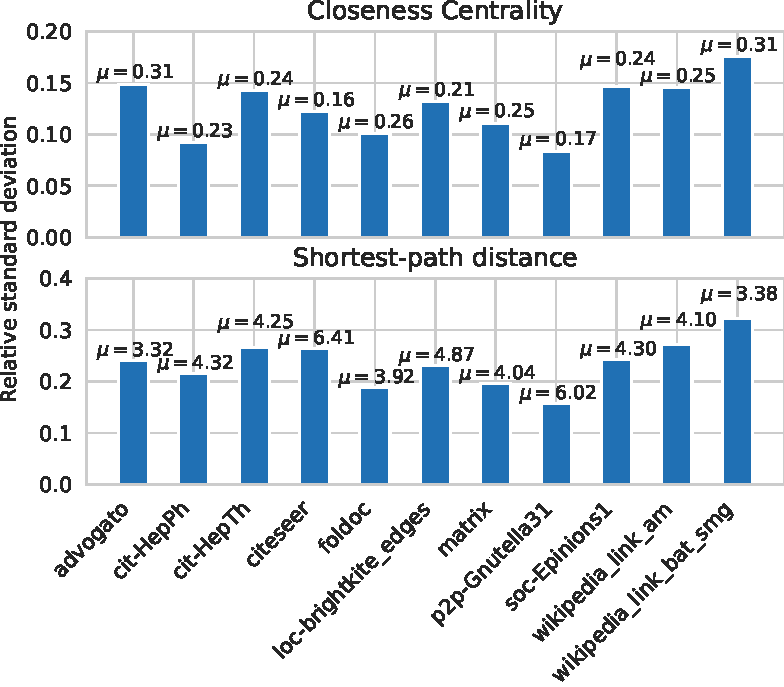
\includegraphics[width=.9\textwidth]{sources/plots/preliminaries/sp-cc-rstd.pdf}
\caption{Relative standard deviation for shortest-paths distances and for
closeness centrality for the networks in \Cref{tab:prelim:insts-rstd}.}
\label{fig:prelim:rstd}
\end{figure}
\end{minipage}\hfill
\begin{minipage}[t]{.5\textwidth}
\centering
\begin{table}[H]
\centering
\setlength{\tabcolsep}{3pt}
\scriptsize
\begin{tabular}{lrrr}
\toprule
Network & $n$ & $m$ & Diameter\\
\midrule
advogato & \numprint{5042} & \numprint{52195} & \numprint{9}\\
cit-HepPh & \numprint{34401} & \numprint{421529} & \numprint{14}\\
cit-HepTh & \numprint{27400} & \numprint{352580} & \numprint{15}\\
citeseer & \numprint{365154} & \numprint{1742596} & \numprint{34}\\
foldoc & \numprint{13356} & \numprint{120238} & \numprint{8}\\
loc-brightkite\_edges & \numprint{56739} & \numprint{212945} & \numprint{18}\\
matrix & \numprint{79116} & \numprint{515397} & \numprint{12}\\
p2p-Gnutella31 & \numprint{62561} & \numprint{147878} & \numprint{11}\\
soc-Epinions1 & \numprint{75877} & \numprint{508836} & \numprint{15}\\
wikipedia\_link\_am & \numprint{20883} & \numprint{105714} & \numprint{12}\\
wikipedia\_link\_bat\_smg & \numprint{21814} & \numprint{123756} & \numprint{13}\\
\bottomrule
\end{tabular}
\caption{Graphs used in \Cref{fig:prelim:rstd} (downloaded from
the public repository KONECT~\cite{kunegis2013konect}).}
\label{tab:prelim:insts-rstd}
\end{table}
\end{minipage}
\end{figure}

\paragraph{Harmonic Centrality}
%
Marchiori and Latora~\cite{marchiori2000harmony} introduced the
\emph{connectivity length} of a graph in order to measure the \emph{efficiency}
of a network in terms of information propagation. The connectivity length of a
graph is defined as the \emph{harmonic mean} of all the pairwise distances
between the vertices in a graph.
Later, harmonic centrality was independently devised by
Dekker~\cite{DBLP:journals/joss/Dekker05} (with the name \enquote{valued
centrality}) and by Rochat~\cite{rochat2009closeness}.
Harmonic centrality is defined as:

\begin{equation}
\label{eq:def:harmonic}
\harm(u) := \sum_{v \in V \setminus \set{u}} \frac{1}{d(u, v)}.
\end{equation}

Under the reasonable assumption that the reciprocal of infinity is zero,
harmonic centrality is well-defined also on disconnected graphs.
%
Further, from an axiomatic point of view, harmonic centrality enjoys several
desirable properties~\cite{DBLP:journals/im/BoldiV14}.


\paragraph{Electrical Closeness}
Electrical closeness~\cite{DBLP:conf/stacs/BrandesF05} --
also known as \emph{current-flow closeness} or \emph{information
centrality}~\cite{stephenson1989rethinking} --
ranks vertices according to their average resistance distance
to the others:
%
\begin{equation}
\label{eq:electrical-closeness}
\elclos(u) := \frac{n - 1}{\sum_{v \in V\change{\setminus\set{u}}} \rdist(u, v)}.
\end{equation}

Analogously to combinatorial closeness, electrical closeness is not directly
applicable to disconnected graphs due to the aforementioned infinite distances
issue. However, generalizations to disconnected graphs such as
Lin's~\cite{lin1976foundations} or Olsen's~\cite{DBLP:conf/icde/OlsenLH14}
apply as well.

Because it takes into considerations all the paths between two vertices,
electrical closeness solves two issues concerning the vertex rankings computed by
combinatorial closeness: (i) having a low discriminative power,
especially on complex networks, and (ii) being
highly susceptible to changes in the graph~\cite{DBLP:journals/it/GrintenAM20}.
These claims are corroborated by the experiments in
Ref.~\cite{DBLP:conf/siamcsc/BergaminiWLM16}.


\paragraph{Forest Closeness}
%
Forest distance closeness centrality (abbreviated with \emph{forest closeness})
is a further variation of closeness centrality where the shortest-path distance
is replaced by the \emph{forest distance}:
%
\begin{equation}
\label{eq:forest-closeness}
\fclosp(u) := \frac{n}{\sum_{v \in V \setminus \set{u}}{\fdistp(u, v)}}.
\end{equation}

The denominator of $\fclosp(u)$ is also called the \emph{forest farness} of $u$.
Compared to other centrality measures, forest closeness presents two main advantages:
(i) by taking all paths into account it has a high discriminative
power~\cite{DBLP:conf/icdm/JinBZ19} and (ii) it handles disconnected
graphs out of the box.

\subsection{Spectral Centrality Measures}
%
\emph{Spectral centrality measures} compute the importance of the vertices of a
graph $G$ by using the left dominant eigenvector of a matrix derived
from a matrix representation of $G$.
The existence and the uniqueness of most of these measures is guaranteed by the
theory developed by Perron and
Frobenius~\cite{perron1907theorie,frobenius1912matrizen} about non-negative
matrices~\cite{DBLP:books/siam/BermanP94}.

\paragraph{Eigenvector Centrality}
Eigenvector centrality implements the idea that a vertex in a network is
important if adjacent to vertices that are themselves important. It can also be
interpreted as an extension of degree centrality where the centrality of a
vertex is \emph{proportional to the centrality of its neighbors}.

Let $\lambda$ be the dominant eigenvalue of the adjacency matrix \Adj of a
graph. Assuming that $V = \set{1, \ldots, n}$, \ie all vertices
in $G$ are indexed from 1 to $n$, the eigenvector centrality
of a vertex $u \in V$ is defined as:
%
\begin{equation}
\label{eq:prelim:eig-centrality}
\eig(u) = \frac 1\lambda\sum_{v = 1}^n A[u,v]\cdot\eig(v),
\end{equation}

In matrix notation, \Cref{eq:prelim:eig-centrality} is equivalent
to $\eig(u) = \vect{x}[u]$ where \vect{x} is the right leading eigenvector
that solves the linear system
$\Adj\vect{x} = \lambda\vect{x}$.

If \Adj is irreducible,\footnote{
A square matrix \mat{M} is called \emph{reducible} if there exists a
permutation matrix \mat{P} such that:
%
\[
\mat{PMP}^{-1} =
\begin{pmatrix}
    \mat{B}_{1,1} & \mat{B}_{1,2}\\
    0 & \mat{B}_{2,2}
\end{pmatrix},
\]
%
where $\mat{B}_{1,1}$ and $\mat{B}_{2,2}$ are non-empty square matrices.
A matrix that cannot be reduced is called \emph{irreducible}.
}
%
the Perron-Frobenius theorem implies that $\lambda > 0$ and that all the
entries of $\vect{x}$ are strictly positive. \Adj is irreducible iff the
corresponding graph is strongly connected~\cite{DBLP:books/siam/BermanP94}. In
case of disconnected graphs, however, the eigenvector centrality of some
vertices could be zero~\cite{newman2018networks}, which makes this measure
suitable for (strongly) connected graphs only.

\paragraph{Katz Centrality}
%
The limitation of eigenvector centrality of being restricted to strongly
connected graphs is resolved by Katz centrality~\cite{katz1953new}. Conversely
to distance-based based centrality measures that only consider shortest paths,
this measure takes into account \emph{all the walks} between two vertices, with
shorter walks having a greater contribution to the centrality score than longer
walks.
%
The Katz centrality of a vertex $u$ is:
%
\begin{equation}
\label{eq:def:katz}
\katz(u) := \sum_{i = 1}^{\infty}\alpha^i \sum_{v\in V} \Adj^i[u, v],
\end{equation}
%
which converges if the \emph{attenuation factor} $\alpha > 0$ is less than the
reciprocal of the largest singular value of \Adj.
Eq.~\eqref{eq:def:katz} can be rewritten in matrix terms:
%
\begin{equation}
\label{eq:def:katz-alg}
\vect{c}_{\text{K}} = \roundb{\roundb{\Ident - \alpha\Adj}^{-1} - \Ident}\ones,
\end{equation}
%
where $\vect{c}_{\text{K}}[u]$ is the Katz centrality of $u\in V$.


\paragraph{PageRank}
Originally designed with the purpose of developing a search engine,
PageRank~\cite{page1999pagerank} is among the most recent and popular spectral
centrality measures.
Despite being tailored to the Internet graph, as of today this measure is used
in applications beyond web graphs~\cite{DBLP:journals/siamrev/Gleich15}.
%
PageRank models the stationary distribution of a random walk over the vertices
of a graph. At any step, the random walk jumps to another random vertex
with probability $1 - \alpha$, where $\alpha \in (0, 1)$ is called
the \emph{damping factor}. The PageRank score of a vertex $u$ is defined as:
%
\[
\pr(u) := \alpha \sum_{v \in N(u)}\frac{\pr(v)}{\deg(v)} + \frac{1 - \alpha}{n}.
\]

\subsection{Path-based Centrality Measures}
\label{sec:prelim:path-based-centrality}
%
Path-based centrality measures take into account all the (shortest) paths hitting
a vertex. Notice that, in unweighted graphs, degree centrality can also be
considered a path-based measure since it evaluates the number of incoming or
outgoing paths of length one.

\paragraph{Betweenness Centrality}
%
Freeman~\cite{freeman1977set} introduced betweenness centrality as a measure of
how much a vertex \emph{controls} the information flow in a network. A vertex
is considered central if it stands \emph{between} other vertices, as it can
control or influence their communications -- under the assumption that
information flows through shortest paths exclusively.
%
More formally, the betweenness centrality of a vertex $u$ is defined as
the probability that a shortest path between any two vertices $x,y \in V
\setminus \set{u}$ passes through $u$.
Let $\sigma_{x,y}$ be the number of shortest paths from $x$ to $y$, and
$\sigma_{x,y}(u)$ be the number of such paths that cross $u$. The betweenness
centrality of $u$ is defined as:
%
\begin{equation}
\label{eq:def:betweenness}
\betw(u) := \sum_{\substack{x,y \in V \setminus \set{u}\\x\neq y,\ \sigma_{x,y} \neq 0}}
\frac{\sigma_{x,y}(u)}{\sigma_{x,y}}.
\end{equation}

Vertices with high betweenness centrality can also be interpreted
as crucial actors whose removal from the network would disrupt most
communications between other vertices~\cite{DBLP:journals/snam/BoldiRV13}.
Indeed, in the example in \Cref{fig:karate-betw}, the removal of
the vertex with highest betweenness (the red one) would isolate six
vertices from the entire network.


\paragraph{\edw Centrality}
Inspired by Katz centrality, in Ref.~\cite{DBLP:conf/alenex/AngrimanGBZGM20}, we
define \edw, a new centrality measure designed to possess two main
properties: (i) to take into consideration \emph{all walks} (not just shortest
paths) of \emph{any length} that cross a vertex and (ii) to admit a natural
generalization to sets of vertices, leading to a monotone and submodular
group centrality measure (see \Cref{sec:group-centrality-measures})
and to a scalable greedy maximization algorithm.

\edw stands for \emph{exponentially decaying walk} as the contribution of a walk
to the centrality score decays exponentially with its length according to
a parameter $\alpha > 0$.
Let $\phi_i(S)$ be the number of $i$-walks (\ie walks of length $i$) that
contain at least one vertex in $S\subseteq V$. The \edw for $u\in V$ is defined
as~\cite{DBLP:conf/alenex/AngrimanGBZGM20}:
%
\[
\ed(u) := \sum_{i = 1}^{\infty}\alpha^i \phi_i(\set{x}).
\]

For the series to converge, $\alpha$ needs to be chosen small enough.
As for Katz centrality, $\alpha$ must be less than the reciprocal of the
largest singular value of the adjacency matrix of the graph~\cite[Sec.
2.2]{DBLP:conf/alenex/AngrimanGBZGM20}.

\section{Group Centrality Measures}
\label{sec:group-centrality-measures}
% Group Closeness
% Group Harmonic
% Group Forest-Closeness
% GED-Walk

The centrality measures we describe in \Cref{sec:centrality-measures} are
also called \emph{single-vertex} centrality measures because they indicate
the importance of a \emph{single} vertex in a graph with respect to the others.
However, determining the centrality of a \emph{group} of vertices \emph{as a whole},
or to find the most central group of vertices -- or group centrality
maximization -- are two frequent problems that arise in graph mining applications
such as influence
maximization~\cite{DBLP:journals/toc/KempeKT15,DBLP:journals/isci/ZhaoWLTG17},
facility
location~\cite{DBLP:journals/pe/GkantsidisMS06,DBLP:conf/icde/LiLCCDZ15},
congestion avoidance~\cite{yan2006efficient}, and others.

Everett and Borgatti~\cite{everett1999centrality} proposed a general
framework to generalize single-vertex centrality measures to groups of
vertices.\footnote{In their work, Everett and Borgatti extended degree,
closeness, betweenness, and flow betweenness centrality to groups of
vertices.} Given a graph $G = (V, E, w)$ a group
centrality measure is a set function $g :
2^V \to \real$ that assigns to each subset of $V$ a group
centrality score. A group centrality measure is a proper
generalization of a single-vertex centrality measure if the two yield the same
score when applied to a group consisting of a single
vertex~\cite{everett1999centrality}.
In general, the vertices in the most central group
\enquote{cover} well the entire graph together; thus, they
often differ considerably from the top-$k$ most individually
central vertices. \Cref{fig:prelim:topk-vs-group} exemplifies this difference
in the closeness centrality case.
The top-$10$ vertices with highest $\clos(\cdot)$ in \Cref{fig:prelim:top-k-cc}
are clustered in the center of the graph and, consequently, far from peripheral
vertices. The set $S$ of $10$ vertices in \Cref{fig:prelim:group-cc}, in turn,
has high \emph{group-closeness}: compared to \Cref{fig:prelim:top-k-cc},
vertices in $S$ are much more scattered around the network and thus the
average distance from a vertex to the nearest in $S$ is lower.

\begin{figure}[t!]
\centering
\begin{subfigure}[t]{.48\textwidth}
\centering
\includesvg[width=.8\textwidth]{euroroad-top-cc-dist}
\caption{Red vertices: top-$k$ vertices with highest closeness.}
\label{fig:prelim:top-k-cc}
\end{subfigure}\hfill
\begin{subfigure}[t]{.48\textwidth}
\centering
\includesvg[width=.8\textwidth]{euroroad-group-cc-dist}
\caption{Red vertices: group of vertices with high
group-closeness (computed with the \growshrink algorithm, see
\Cref{ch:group-closeness-local-search}).}
\label{fig:prelim:group-cc}
\end{subfigure}
\caption{Comparison between top-$k$ closeness centrality and group-closeness centrality
($k = 10$) on the European road network~\cite{DBLP:journals/corr/abs-1106-5524}
(downloaded from the public repository KONECT~\cite{kunegis2013konect} and
drawn with the Fruchteman Reingold algorithm~\cite{DBLP:journals/spe/FruchtermanR91}).
Red vertices represent in \Cref{fig:prelim:top-k-cc} the top-$k$ vertices
with highest closeness and, in \Cref{fig:prelim:group-cc}, the $k$ vertices in
a set with high group-closeness centrality. For the other vertices, the
bluest they are the greater is their distance to the nearest red vertex.
Images were generated with the Gephi software~\cite{DBLP:conf/icwsm/BastianHJ09}.}
\label{fig:prelim:topk-vs-group}
\end{figure}

\paragraph{Properties of Set Functions}
Properties of set functions such as monotonicity and submodularity have played
a crucial role in combinatorial
optimization~\cite{DBLP:journals/siamcomp/FeigeMV11,DBLP:conf/focs/Vondrak09,
DBLP:conf/ismp/Lovasz82,DBLP:journals/mp/NemhauserWF78}.

\begin{definition}[Monotonicity]
\label{def:perlim:monotonicity}
Let $X$ be a non-empty finite set.
A set function $f : 2^V \to \real$ is called
\emph{non-decreasing} if $f(T) \ge f(S)$ for all $T \supseteq S$.
Similarly, $f$ is called \emph{non-increasing} if for every
$S \subseteq T$, we have $f(S) \ge f(T)$.
In both cases, $f$ is called \emph{monotone}.
\end{definition}

\begin{definition}[Submodularity and Marginal Gain]
\label{def:perlim:submodularity}
A set function $f : 2^X \to \real$ is called
\emph{submodular} if, for every $S \subseteq T \subseteq X$ and every $x \in X
\setminus T$, we have that:
%
\[
f(S \cup \set{x}) - f(S) \ge f(T \cup \set{x}) - f(T \cup \set{x}).
\]

In this context, the value $f(S \cup \set{x}) - f(S)$ is
called the \emph{marginal gain} of $x$ \wrt the set $S$.
%
Similarly, $f$ is called \emph{supermodular} if $f(S \cup \set{x}) - f(S) \le
f(T \cup \set{x}) - f(T)$ for every $S \subseteq T \subseteq X$ and
every $x \in X \setminus T$.
\end{definition}

The relevance of these properties stems from a classical result
about optimization of monotone and submodular set function:

\begin{proposition}[\cite{DBLP:journals/mp/NemhauserWF78}]
\label{prop:prelim:greedy-apx}
Let $f : 2^X \to \real$ be a non-decreasing submodular set function.
Consider the problem of maximizing $f$ over all possible subsets
$S \subseteq X$ \wrt the cardinality constraint $|S| \le k$ for
some $k \in \natn$. Let $S^\star$ be the optimal solution to this
problem:
%
\[
    S^\star := \argmax_{S \subseteq X, |S| \le k}f(S).
\]

The greedy algorithm that constructs $S$ by iteratively
adding the element $x \in X$ with highest marginal gain
$f(S, x) := f(S \cup \set{x}) - f(S)$ to $S$ yields a
$(1 - 1/e)$-approximation for this problem. Specifically,
if $\tilde{S}$ is the result of the greedy algorithm, it holds
that $f(\tilde{S}) \ge (1 - 1/e)f(S^\star)$.
\end{proposition}

\paragraph{Group-Degree Centrality}
The \emph{group-degree centrality} of a group $S\subset V$ is the number
of vertices in $V\setminus S$ that are neighbors of at least a vertex in
$S$~\cite{everett1999centrality}:
%
\[\gdeg(S) := \left|\set{v \in V \setminus S : (u, v)\in E\ \text{for some}\ u \in S}\right|.\]
%
%Because this quantity alone is often meaningless, Everett and Borgatti
%propose to divide it by the number of non-group vertices, ensuring
%the values of group degree to be in $[0, 1]$.
%
It is simple to verify that group-degree is not monotone: in a triangular
graph the group-degree of a single vertex is two, whereas the group-degree
of any set with two vertices is one.
On the other hand, group-degree is submodular.

\begin{lemma}
Group-degree is submodular.
\end{lemma}

\begin{proof}
Let $\delta_u(S)$ be 1 if $\set{u, v} \in E$ for some $v \in S$, 0 otherwise.
We need to show that $\gdeg(S \cup \set{u}) - \gdeg(S) \ge \gdeg(T \cup
\set{u}) - \gdeg(T)$. Because $T \supseteq S$ it holds that:
%
\[\gdeg(S \cup \set{u}) - \gdeg(S) = |N(u) \setminus S| - \delta_u(S) \ge
|N(u) \setminus T| - \delta_u(T) = \gdeg(T \cup \set{u}) - \gdeg(T).\]
%
\end{proof}

\paragraph{Group-Closeness Centrality}
For a group $S \subset V$, its \emph{group-closeness centrality} is
defined as~\cite{DBLP:conf/alenex/BergaminiGM18}:
\begin{equation}
\label{eq:prelim:gclos}
\gclos(S) := \frac{n}{\sum_{v \in V \setminus S} d(S, v)},
\end{equation}
%
where $d(S, v)$ is $\min_{s \in S}d(s, v)$, see \Cref{eq:def:dist-point-set}.
The denominator of $\gclos(S)$ is also called the \emph{group-farness}
of $S$.
%
As with closeness centrality, group-closeness is only defined on
strongly connected graphs. Further, it is easy to see that $\gclos(\cdot)$ is
monotone: for each $S \subseteq T \subset V$ and $u \in V \setminus T$
we have that $d(T, u) \le d(S, u)$, and thus $\gclos(T) \ge \gclos(S)$.
However, group-closeness is not submodular, and this can be demonstrated with a
simple counterexample.

\begin{lemma}
\label{lemma:prelim:gclos-not-submod}
Group-closeness is not submodular.
\end{lemma}
\begin{proof}
Consider a complete undirected graph with five vertices
numbered from 0 to 4, let $S = \set{0, 1}$, $T = \set{0, 1, 2}$, and $v = 3$:
%
\[
\gclos(S\cup\set{v}) - \gclos(S) = \frac 52 - \frac 53 = \frac 56 < \gclos(T
\cup \set{v}) - \gclos(T) = \frac 51 - \frac 52 = \frac 52.\qedhere
\]
%
\end{proof}

\paragraph{Group-Harmonic Centrality}
The \emph{group-harmonic centrality} of a group $S \subset V$ is
defined as~\cite{DBLP:conf/alenex/AngrimanBDGGM21}:
%
\[\gharm(S) := \sum_{v\in V\setminus S} \frac{1}{d(S, v)},\]
%
where, as for $\harm(\cdot)$, $1/d(S,v) = 0$ if no vertex in $S$ reaches $v$.
Hence, group-harmonic also handles disconnected graphs. This measure is
submodular but not
monotone~\cite{DBLP:conf/alenex/AngrimanBDGGM21}.
Although such a definition is a natural generalization of harmonic centrality
to groups of vertices, the way it handles vertices in the group may seem
questionable. Indeed, vertices in $S$ count as 0 in the harmonic centrality
score of $S$ while they are the closest ones to $S$.
%
On the other hand, assigning them an arbitrary value greater than 0 would
be unsatisfactory. A workaround for this problem is to always compare the
group-harmonic centrality of groups with equal cardinality, so that the
value assigned to vertices in the group does not have any
impact~\cite{DBLP:conf/alenex/AngrimanBDGGM21}.

\paragraph{GED-Walk Centrality}
%
As described in \Cref{sec:centrality-measures}, \edw was designed to
naturally generalize to groups of vertices $S \subseteq V$. This leads us to
GED-Walk:
%
\[
\ged(S) := \sum_{i = 1}^{\infty}\alpha^i \phi_i(S).
\]

As we show in \Cref{ch:ged-walk}, GED-Walk not only is both monotone and
submodular, but it is also faster to maximize (for groups of small size) than
existing shortest-path based group centrality measures.


\section{Matchings}
\label{sec:prelim:matchings}
%
Let $G = (V, E, w)$ be an undirected weighted graph. A \emph{matching} in $G$
is a subset of pairwise disjoint edges $M \subseteq E$. A vertex
is called \emph{matched} in $M$ if it is incident to an edge $e \in M$;
otherwise, it is called \emph{free} or \emph{unmatched}.
%
A matching $M$ is called \emph{maximal} if no further edge can be added to
$M$ while retaining the matching property, and \emph{maximum} if no other
matching with higher cardinality exists.
%
Computing a maximum cardinality matching (or MCM) of a graph is a popular
combinatorial optimization problem that can be solved in $\Oh(m\sqrt{n})$
by the algorithm of Micali and Vazirani~\cite{DBLP:conf/focs/MicaliV80}.
By restricting the input algorithms to planar graphs, MCM can be solved in
$\Oh(n^{\omega})$~\cite{DBLP:journals/algorithmica/MuchaS06}.

The weight of a matching $M$ is the sum of the weights of the edges in $M$
and a maximum \emph{weighted} matching (or MWM) is a matching with maximum weight.
The fastest known algorithm for finding a MWM is by Galil
\etal~\cite{galil1986efficient} and it takes $\Oh(mn\log{n})$ time. Algorithms
for MWM with lower time complexity exist
but they are specialized for bipartite graphs~\cite{DBLP:journals/tcs/Sankowski09}
or graphs with integral edge weights~\cite{DBLP:journals/jacm/GabowT91}.
%
A broader overview over matching theory and algorithms is provided in
Refs.~\parencites[Ch. 5][]{bisseling2020parallel,lovasz2009matching}.


\section{Dynamic Graphs}
\label{sec:prelim-dynamic-graphs}
% Describe model, events, fully-dynamic vs semi-dynamic.
% Snapshots, batch vs single
So far we only considered \emph{static} graphs, \ie graphs
that do not change over time.
However, graphs that occur in real-world scientific and commercial applications
are often \emph{dynamic}, \ie they evolve over time: vertices and edges are
inserted, removed, or edge weights are updated. Examples include social network
analysis~\cite{DBLP:conf/icdm/ZhuangSTZS13}, computational
biology~\cite{DBLP:conf/compgeom/EyalH05}, advertisements on search
engines~\cite{DBLP:conf/focs/MehtaSVV05} and many more.

We target \emph{fully-dynamic} graphs, \ie dynamic graphs
where update operations are restricted to edge insertions and
removals~\cite{DBLP:books/crc/99/EppsteinGI99}.\footnote{On weighted graphs,
edge weight updates can be represented as an edge removal followed by an edge
insertion.} These operations are also called \emph{edge updates}.
More formally, let $G = (V, E, w)$ be a graph; an edge update is an operation
that transforms $G$ into another graph $G' = (V, E', w')$.
In case of the insertion of an edge $(u, v) \notin E$ with weight $\alpha$, we
have that $E' = E \cup \set{(u, v)}$, $w'(e) = w(e)$ for all $e \in E$ and
$w'(u, v) = \alpha$.
Conversely, in case of the removal of an edge $(u, v) \in E$, we have that
$E' = E \setminus \set{(u, v)}$ and $w'(e) = w(e)$ for all $e \in E'$.
Further, we denote with superscript $'$ any additional property of the graph $G'$,
\eg $d'(u, v)$ is the shortest-path distance from $u$ to $v$ in $G'$.


\section{Performance and Quality Indicators}
\label{sec:prelim-performance-quality}
%
An algorithm's performance is commonly measured by its \emph{running time}
and the wall-clock time is a widely used indicator for running time. For
solution quality, indicators are usually problem-specific; we often measure the
gap between the algorithm's solution and the optimum, if known, or a highly
accurate solution.
In the following, we describe the indicators we use in our experiments to
evaluate the performance and the solution quality of our algorithms.

\paragraph{Running Time}
We often compare the running time of two algorithms $A$ and $B$ on several
instances. As recommended in Ref.~\cite{DBLP:journals/algorithms/AngrimanGLMNPT19},
in order to make a concise evaluation, we aggregate the wall-clock times over
\emph{ratios}, which means computing the \emph{algorithmic speedup} of
$A$ \wrt $B$. For a fair comparison of the algorithmic
aspects, the algorithmic speedup is often measured over the \emph{sequential}
executions of the algorithms -- \ie using a single thread.
To summarize multiple algorithmic speedup values we use the geometric
mean~\cite{DBLP:journals/ior/Bixby02}:
%
\[
\gmean(\text{speedup}) =
\roundb{\prod_{i = 1}^{\text{\# of values}}
\text{speedup on instance}\ i}^{\frac{1}{\text{\# of values}}}
\]
%
as it has the fundamental property that
$\gmean(\text{speedup}) =
\frac{\gmean(\text{running times of}\ A)}{\gmean(\text{running times of}\ B)}$.

Concerning parallel algorithms, we evaluate how efficiently they can be
parallelized. To do so we use the \emph{parallel speedup} of an algorithm $A$,
\ie the speedup of a parallel execution of $A$ over its sequential execution.

\paragraph{Solution Quality}
%
The quality of the results yielded by the algorithms we consider in this work is
represented by either a scalar, a vector of scores, or a ranking.
The first category concerns problems such as group centrality maximization:
the solution is a set $S$ of vertices and its quality is the group centrality
score of $S$.
In this case, we measure the gap between the computed solution and the optimum
as a percentage and we aggregate multiple results with the geometric
mean.\footnote{If the optimum is too computationally expensive to compute, we
resort to high-quality approximations of it.}

In the second category, we have solutions where a score is computed for each vertex
(or edge) in the graph. Let us assume that all vertices in the graph are
indexed from $1$ to $n$, let $\widetilde{\vect{x}}$ be the computed vector (where
$\widetilde{\vect{x}}[i]$ is the score computed for the $i$-th vertex) and let
$\vect{x}$ be vector of the exact scores. Recall the definition of a vector
norm.

\begin{definition}[Vector Norm~\cite{pugh2002real}]
Let $Z$ be a vector space over $\real$. A vector norm on $Z$ is a function
$\norm{\cdot} : Z \to \real$ such that:
\begin{enumerate}
    \item for each $\vect{z}\in Z$, $\norm{\vect{z}} \ge 0$ and $\norm{\vect{z}} = 0
        \Leftrightarrow \vect{z} = 0$;

    \item for each $\vect{z} \in Z$ and every $\alpha\in\real$, $\norm{\alpha \vect{x}}
        = |\alpha|\cdot\norm{\vect{x}}$;

    \item for each $\vect{z}_1, \vect{z}_2\in Z$, $\norm{\vect{z}_1 + \vect{z}_2} \le
        \norm{\vect{z}_1} + \norm{\vect{z}_2}$ (triangle inequality).

\end{enumerate}
\end{definition}

For error estimation purposes, we are interested in three vector norms on
$\real^n$, the 1-norm, the 2-norm, and the max-norm, which are defined as
follows for a vector $\vect{z} \in \real^n$~\cite{pugh2002real}:

\begin{alignat*}{2}
    &\onenorm{\vect{z}} &&:= \sum_{i = 1}^n|\vect{z}[i]|,\\
    &\twonorm{\vect{z}} &&:= \sqrt{\sum_{i = 1}^n \vect{z}[i]^2},\\
    &\maxnorm{\vect{z}} &&:= \max(|\vect{z}[1]|, |\vect{z}[2]|, \ldots, |\vect{z}[n]|).
\end{alignat*}

Depending on the problem under consideration and the algorithm's quality
guarantees, we evaluate the gap between the computed result
$\xapprox$ and the baseline $\vect{x}$ on the basis of the 1-norm, 2-norm, and/or
the max-norm of the absolute
error vector $(|\xapprox[1] - \vect{x}[1]|, \ldots, |\xapprox[n] - \vect{x}[n]|)$
and/or of the relative error vector $\roundb{\frac{|\xapprox[1] -
\vect{x}[1]|}{\vect{x}[1]}, \ldots, \frac{|\xapprox[n] - \vect{x}[n]|}{\vect{x}[n]}}$.

Finally, the third category accounts for solutions where the quality is measured
by a ranking of the vertices according to their individual scores, which is often
more relevant than the scores per se~\cite{DBLP:conf/faw/OkamotoCL08,newman2018networks}.
As we did above, let $\vect{x}$ be the vector of exact scores (or a high-quality
approximation of it) and let $\widetilde{\vect{x}}$ be the vector of the computed
scores.
A pair of scores $\left<(\vect{x}[i], \widetilde{\vect{x}}[i]), (\vect{x}[j], \widetilde{\vect{x}}[j])\right>$
with $i < j$ is said to be \emph{concordant} if either
$(\vect{x}[i] > \vect{x}[j]) \wedge (\widetilde{\vect{x}}[i] >
\widetilde{\vect{x}}[j])$ or $(\vect{x}[i] < \vect{x}[j]) \wedge (\widetilde{\vect{x}}[i] <
\widetilde{\vect{x}}[j])$, ties are neglected for simplicity; otherwise, they are said to be \emph{discordant}.
We measure the quality of a ranking it terms of:
\begin{itemize}
    \item Percentage of concordant pairs:
    \[
    \frac{\text{\# of concordant pairs}}{{n \choose 2}};
    \]
    \item Kendall $\tau$ coefficient:
    \[
        \tau := \frac{(\text{\# of concordant pairs}) - (\text{\# of discordant pairs})}{{n \choose 2}}.
    \]
\end{itemize}
